\chapter{Acerca de la implementación de TexToES}

\label{AppendixA}

TexToES fue programado con Python 2.7.9 y con la ayuda de librerias como xml.etree, ConfigObj y request. Cada una de las tres librerías pueden instalarse con pip.
A continuación se lista la organización del directorio que contiene la solución.

\begin{lstlisting}[basicstyle=\scriptsize]
+ TexToES
  | corpus
  + - forms_data
    - hitl_responses
    - hjudgement
    - corpus.txt
    - parsed_responses.txt
    - summarized_corpus.txt
  | tesis_document_sourcecode
  + - Appendices
    - Chapters
    - Figures
    - TexToES - Thur Luis - Trabajo Final.pdf
    - TexToES - Thur Luis - Trabajo Final.tex
  + evidencia.txt
  + language.template
  + lenguage_evaluator.py
  + lenguage_generator.py
  + LICENCE
  + mathml_client.py
  + module.py
  + preprocessor.py
  + test_module.py
\end{lstlisting}

La carpeta \textbf{corpus} contiene lo necesario para evaluar la transcripcion, dentro contiene los siguientes elementos:
\begin{itemize}
\item forms\_data: Contiene los archivos CSV con las respuestas de los voluntarios que contestaron como leerian las formulas matematicas.
\item hitl\_responses: Contiene los archivos CSV con las respuestas de los voluntarios que participaron en la evaluacion de retrotraduccion
\item hjudgement: Contiene los archivos CSV con las respuestas de los jueces  que evaluaron las transcripciones de TexToES
\item corpus.txt: Archivo que contiene todas las reglas gramaticales atomicas presentes en los archivos .CSV en forms\_data
\item parsed\_responses.txt: Contiene todas las respuestas CSV en forms\_data procesadas
\item summarized\_corpus.txt: Contiene las ocurrencias de reglas gramaticales atomicas con la correspondencia anotada de la etiqueta CMathML a la cual se relaciona
\end{itemize}

También tenemos una carpeta donde se encuentra todo el código usado para generar el pdf de éste documento, puede ser encontrado en textbf{tesis\_document\_sourcecode}, ésta contiene los siguientes elementos:
\begin{itemize}
\item Appendices: Apendices de la tesis
\item Chapters: Capitulos de la tesis
\item Figures: Figuras de la tesis
\item TexToES - Thur Luis - Trabajo Final.pdf: Documento principal de tesis en formato pdf.
\item TexToES - Thur Luis - Trabajo Final.tex: Documento principal de tesis en format tex para editar.
\end{itemize}

Finalmente, en la carpeta raíz tenemos los siguientes elementos.

\begin{itemize}
\item evidencia.txt: Aqui se listan todas las transcripciones que TexToES ha hecho desde el inicio, sirve para regresionar sobre TexToES cuando alguna funcionalidad nueva se agrega.
\item test\_module.py: Modulo de testing para regresionar.
\item module.py: Modulo principal de TexToES, se utiliza para obtener la transcripcion para una expresion matematica.
\item mathml\_client.py: Cliente que se comunica con SnuggleTeX, es alimentado por module.py si vino como entrada un string latex. Obtiene el CMathML asociado, y alimenta a preprocessor.py
\item preprocessor.py: Dada una formula matematica CMathML va a generar el stack que luego alimentará a lenguage\_generator.py para ir obteniendo las traducciones.
\item lenguage\_generator.py: Se encarga de traducir las partes mas atomicas de la expresion matematica, procesa el stack que recibe de preprocessor.py
\item language.template: Contiene todas las reglas de transcripciones, usadas por language\_generator.py
\item lenguage\_evaluator.py: Se encarga de darle un puntaje a las transcripciones basado en los datos que hay en forms\_data
\item LICENCE, licencia de TexToES
\end{itemize}

Aqui podemos observar el diagrama de clases de la implementación de TexToES.

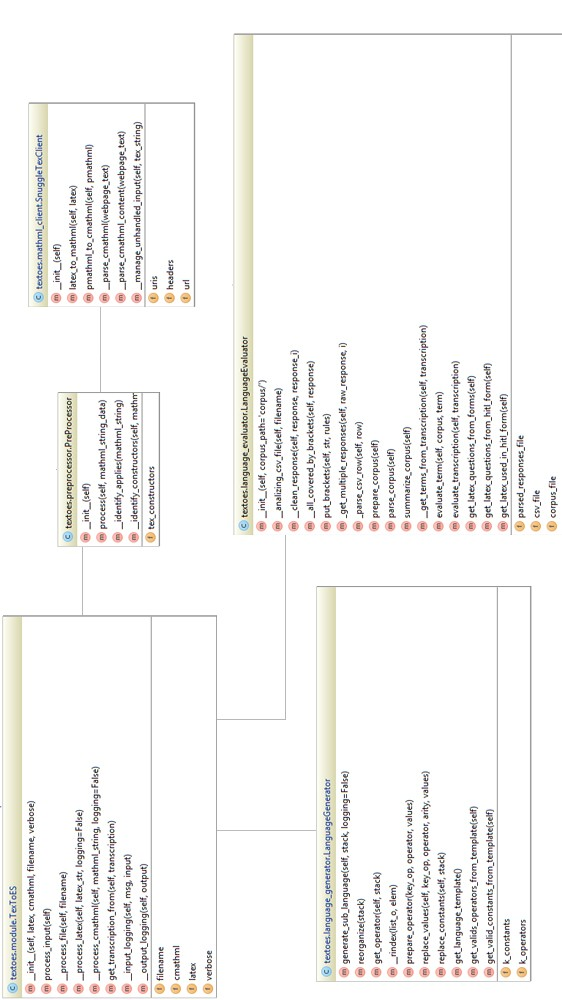
\includegraphics[width=11.24cm, height=20cm]{figures/diagram.jpg}

Finalmente, usted puede consultar el código fuente en GitHub\footnote{https://github.com/lthurr/textoes}. Los comentarios inline en el código puede ayudarle a entender mucho mejor la implementación.
